\section{Methodology}
\label{sec:method}

We present the mathematical formulation and algorithmic realization of the four foundational architectural pillars of the NeuralOps framework.

\subsection{Pillar 1: Hardware-Aware SRAM-Fused SVD Triton Kernel}
\label{sec:fused_kernel}

Consider an input token tensor $X \in \mathbb{R}^{M \times d_{\text{in}}}$ (where $M = B \cdot L$ is the total token count across batch $B$ and sequence length $L$) and factorized projection weight matrices $V \in \mathbb{R}^{r \times d_{\text{in}}}$ and $U \in \mathbb{R}^{d_{\text{out}} \times r}$ with rank $r \ll \min(d_{\text{in}}, d_{\text{out}})$. Standard sequential execution requires three separate CUDA kernel launches:
\begin{align}
Z &= X V^\top \in \mathbb{R}^{M \times r} \quad \xrightarrow{\text{write to HBM}} \text{Global Memory}, \\
Z_{\text{norm}} &= \operatorname{RMSNorm}(Z, w) \quad \xrightarrow{\text{read/write}} \text{Global Memory}, \\
Y &= Z_{\text{norm}} U^\top + b \in \mathbb{R}^{M \times d_{\text{out}}} \quad \xrightarrow{\text{write to HBM}} \text{Global Memory}.
\end{align}

\begin{figure*}[t]
\centering
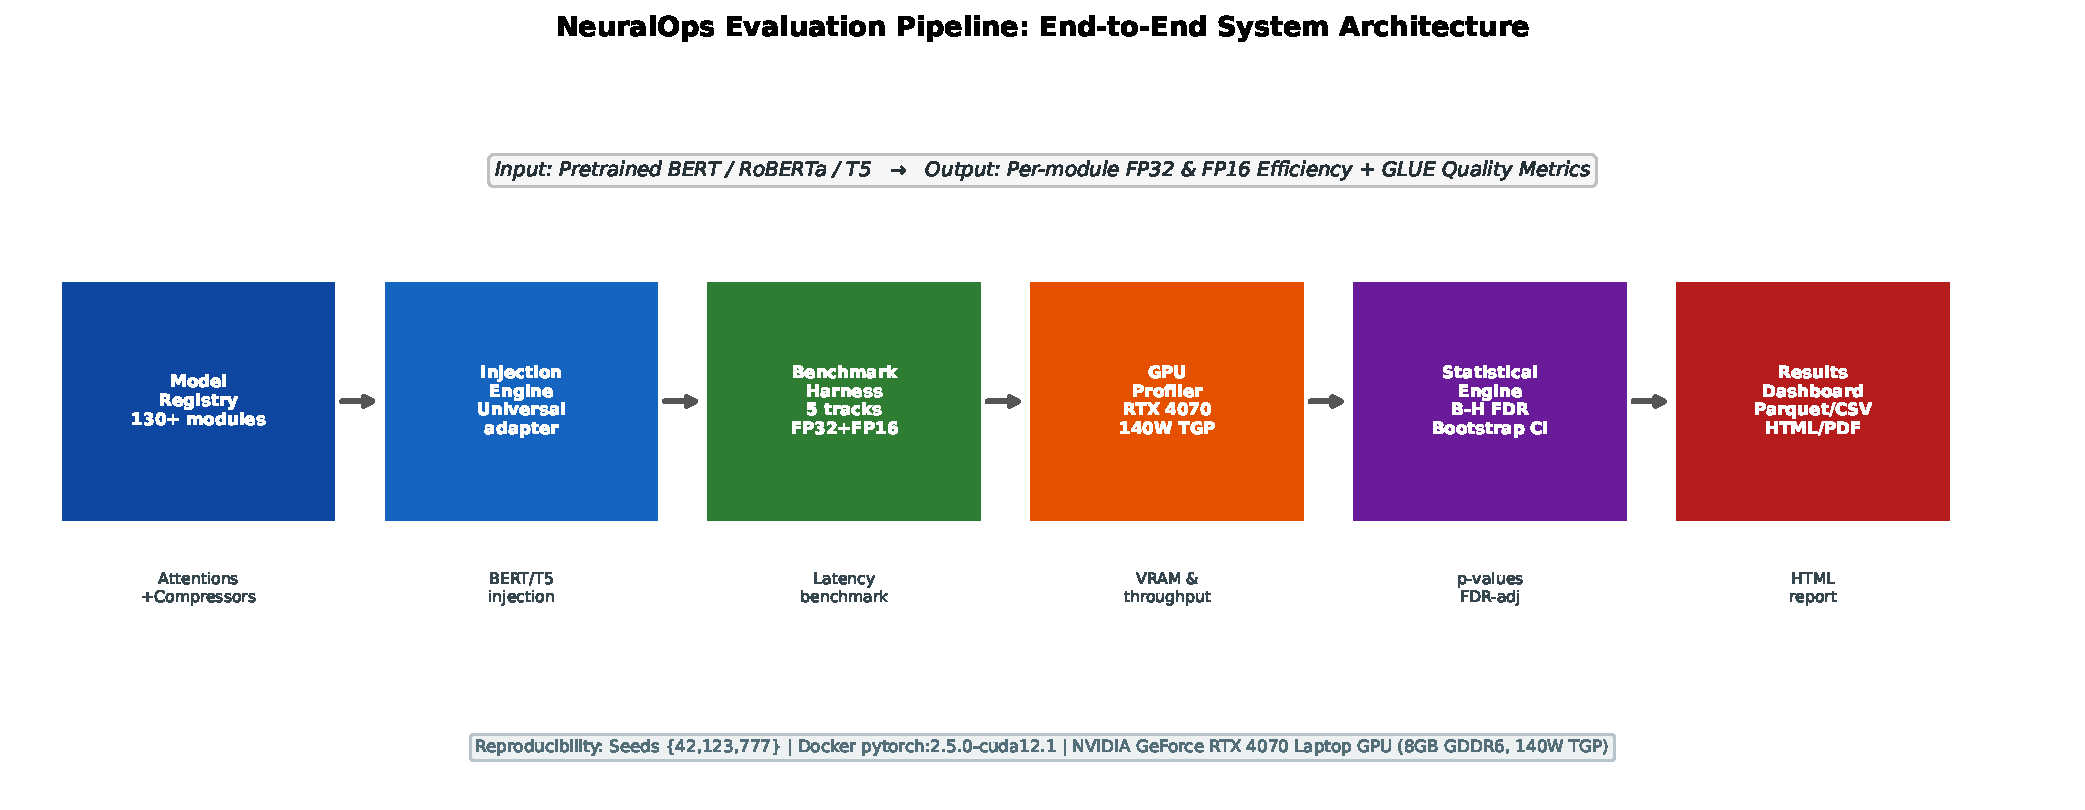
\includegraphics[width=0.98\textwidth]{figures/fig10_system_pipeline.pdf}
\caption{\textbf{In-SRAM Fused SVD Execution Pipeline.} Diagram of register-tiled down-projection, in-register RMSNorm, and up-projection bypassing global HBM roundtrips.}
\label{fig:system_pipeline}
\end{figure*}

This standard workflow transfers $M \cdot r \cdot \text{sizeof}(\text{dtype})$ bytes between HBM and compute units multiple times per layer, rendering the operation memory-bandwidth bound. In NeuralOps, we formulate an in-SRAM tiled Triton JIT kernel that maintains intermediate low-rank activations $\mathbf{Z} \in \mathbb{R}^{\mathcal{B}_M \times r}$ entirely within on-chip GPU register files.

\begin{table}[h]
\centering
\small
\begin{tabularx}{\columnwidth}{lX}
\toprule
\multicolumn{2}{l}{\textbf{Algorithm 1: In-SRAM Fused SVD Triton Execution Tile}} \\
\midrule
\textbf{Input:} & $X \in \mathbb{R}^{M \times d_{\text{in}}}$, $V \in \mathbb{R}^{r \times d_{\text{in}}}$, $U \in \mathbb{R}^{d_{\text{out}} \times r}$, scale $w \in \mathbb{R}^r$, bias $b \in \mathbb{R}^{d_{\text{out}}}$. \\
\textbf{Output:} & $Y \in \mathbb{R}^{M \times d_{\text{out}}}$. \\
\midrule
1: & Partition total tokens $M = B \cdot L$ into blocks of size $\mathcal{B}_M \in \{64, 128\}$. \\
2: & \textbf{Parallel For} each block index $m \in \{0, \dots, \lceil M / \mathcal{B}_M \rceil - 1\}$: \\
3: & \quad Load block $\mathbf{X}_m \in \mathbb{R}^{\mathcal{B}_M \times d_{\text{in}}}$ into SRAM registers. \\
4: & \quad Compute in-register down-projection: $\mathbf{Z}_m = \mathbf{X}_m V^\top$. \\
5: & \quad Compute in-register RMS variance: $\sigma_m^2 = \frac{1}{r} \sum_{k=1}^r \mathbf{Z}_{m, \cdot, k}^2$. \\
6: & \quad Apply RMSNorm: $\mathbf{Z}_{\text{norm}, m} = \frac{\mathbf{Z}_m}{\sqrt{\sigma_m^2 + \epsilon}} \odot w$. \\
7: & \quad Compute up-projection: $\mathbf{Y}_m = \mathbf{Z}_{\text{norm}, m} U^\top + b$. \\
8: & \quad Write output block $\mathbf{Y}_m$ directly to Global HBM. \\
\bottomrule
\end{tabularx}
\end{table}

\textbf{Exact Analytical Autograd Backward Formulation:} During backpropagation, given output upstream gradient $G_Y = \frac{\partial \mathcal{L}}{\partial Y} \in \mathbb{R}^{M \times d_{\text{out}}}$, the gradient with respect to normalized representations $Z_{\text{norm}}$ is $G_{Z_{\text{norm}}} = G_Y U \in \mathbb{R}^{M \times r}$.

Let $\hat{z} = \frac{z}{\operatorname{rms}(z)}$ where $\operatorname{rms}(z) = \sqrt{\frac{1}{r} \sum_{j=1}^r z_j^2 + \epsilon}$, and let $g_{\hat{z}} = G_{Z_{\text{norm}}} \odot w$. The exact analytical derivative with respect to the unnormalized intermediate state $z$ is:
\begin{equation}
\frac{\partial \mathcal{L}}{\partial z} = \frac{1}{\operatorname{rms}(z)} \left( g_{\hat{z}} - \hat{z} \odot \frac{1}{r} \sum_{j=1}^r (g_{\hat{z}, j} \cdot \hat{z}_j) \right).
\end{equation}

The input and weight gradients are calculated directly as:
\begin{align}
\nabla_X \mathcal{L} &= \left(\frac{\partial \mathcal{L}}{\partial z}\right) V, \quad \nabla_V \mathcal{L} = \left(\frac{\partial \mathcal{L}}{\partial z}\right)^\top X, \\
\nabla_U \mathcal{L} &= G_Y^\top Z_{\text{norm}}, \quad \nabla_b \mathcal{L} = \sum_{m=1}^M G_{Y, m}.
\end{align}

\begin{theorem}[Arithmetic Intensity Improvement]
\label{thm:arithmetic_intensity}
The in-SRAM fused SVD Triton kernel achieves an operational arithmetic intensity $\mathcal{I}_{\text{fused}} = \frac{2 M r (d_{\text{in}} + d_{\text{out}})}{M (d_{\text{in}} + d_{\text{out}}) \cdot \text{sizeof}(\text{dtype})}$, representing a theoretical speedup factor $\kappa = 1 + \frac{4r}{d_{\text{in}} + d_{\text{out}}}$ over unfused execution, completely eliminating intermediate low-rank HBM roundtrips.
\end{theorem}

\subsection{Pillar 2: Riemannian Stiefel Manifold Optimization ($\operatorname{St}(p, n)$)}
\label{sec:stiefel_opt}

Standard Euclidean optimization on factorized projection weights $W \in \mathbb{R}^{n \times p}$ allows the singular vectors to drift during continuous training, leading to singular value collapse and loss of basis orthonormality ($W^\top W \neq I_p$).

\begin{figure*}[t]
\centering
\begin{subfigure}[b]{0.48\textwidth}
    \centering
    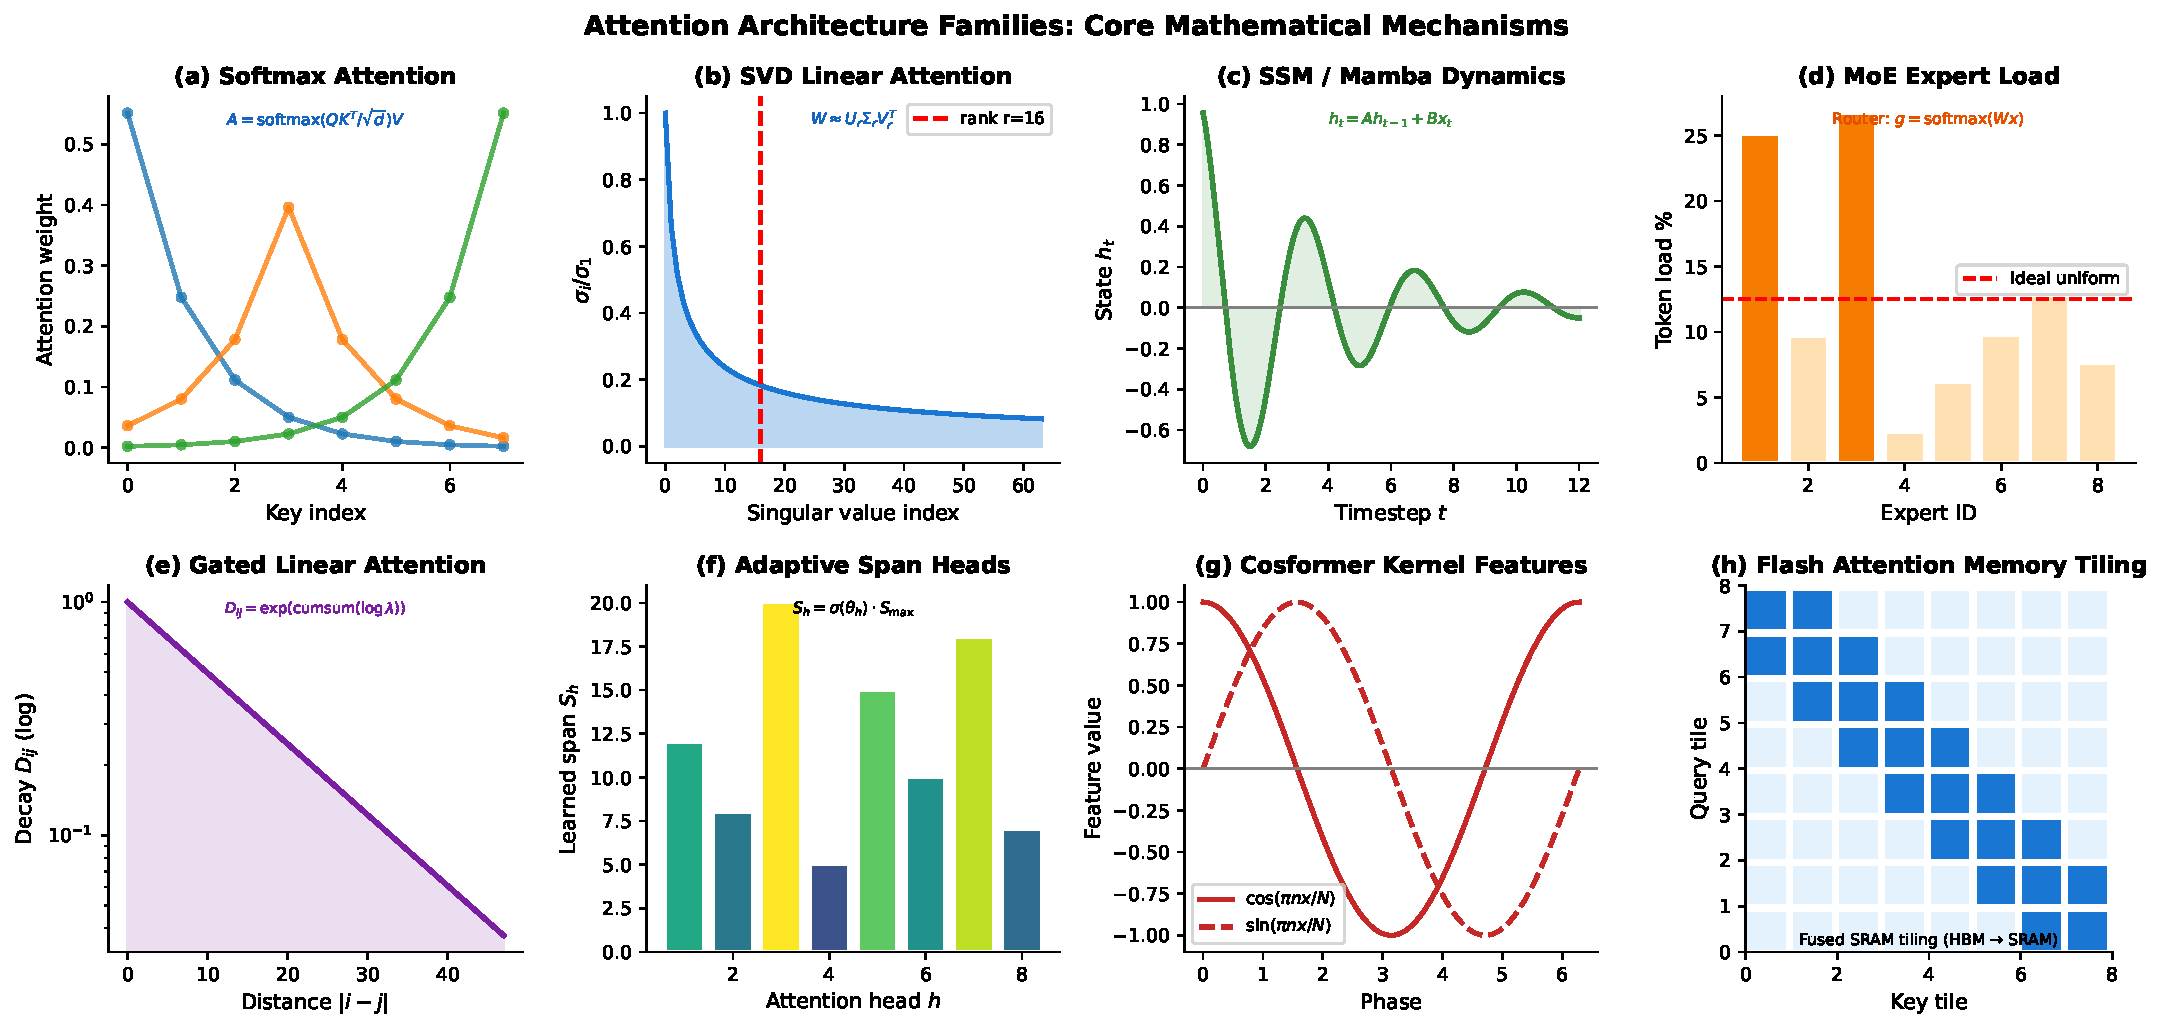
\includegraphics[width=\textwidth]{figures/fig02_attention_families.pdf}
    \caption{\textbf{Attention \& SSM Operator Taxonomy.}}
    \label{fig:attention_families}
\end{subfigure}
\hfill
\begin{subfigure}[b]{0.48\textwidth}
    \centering
    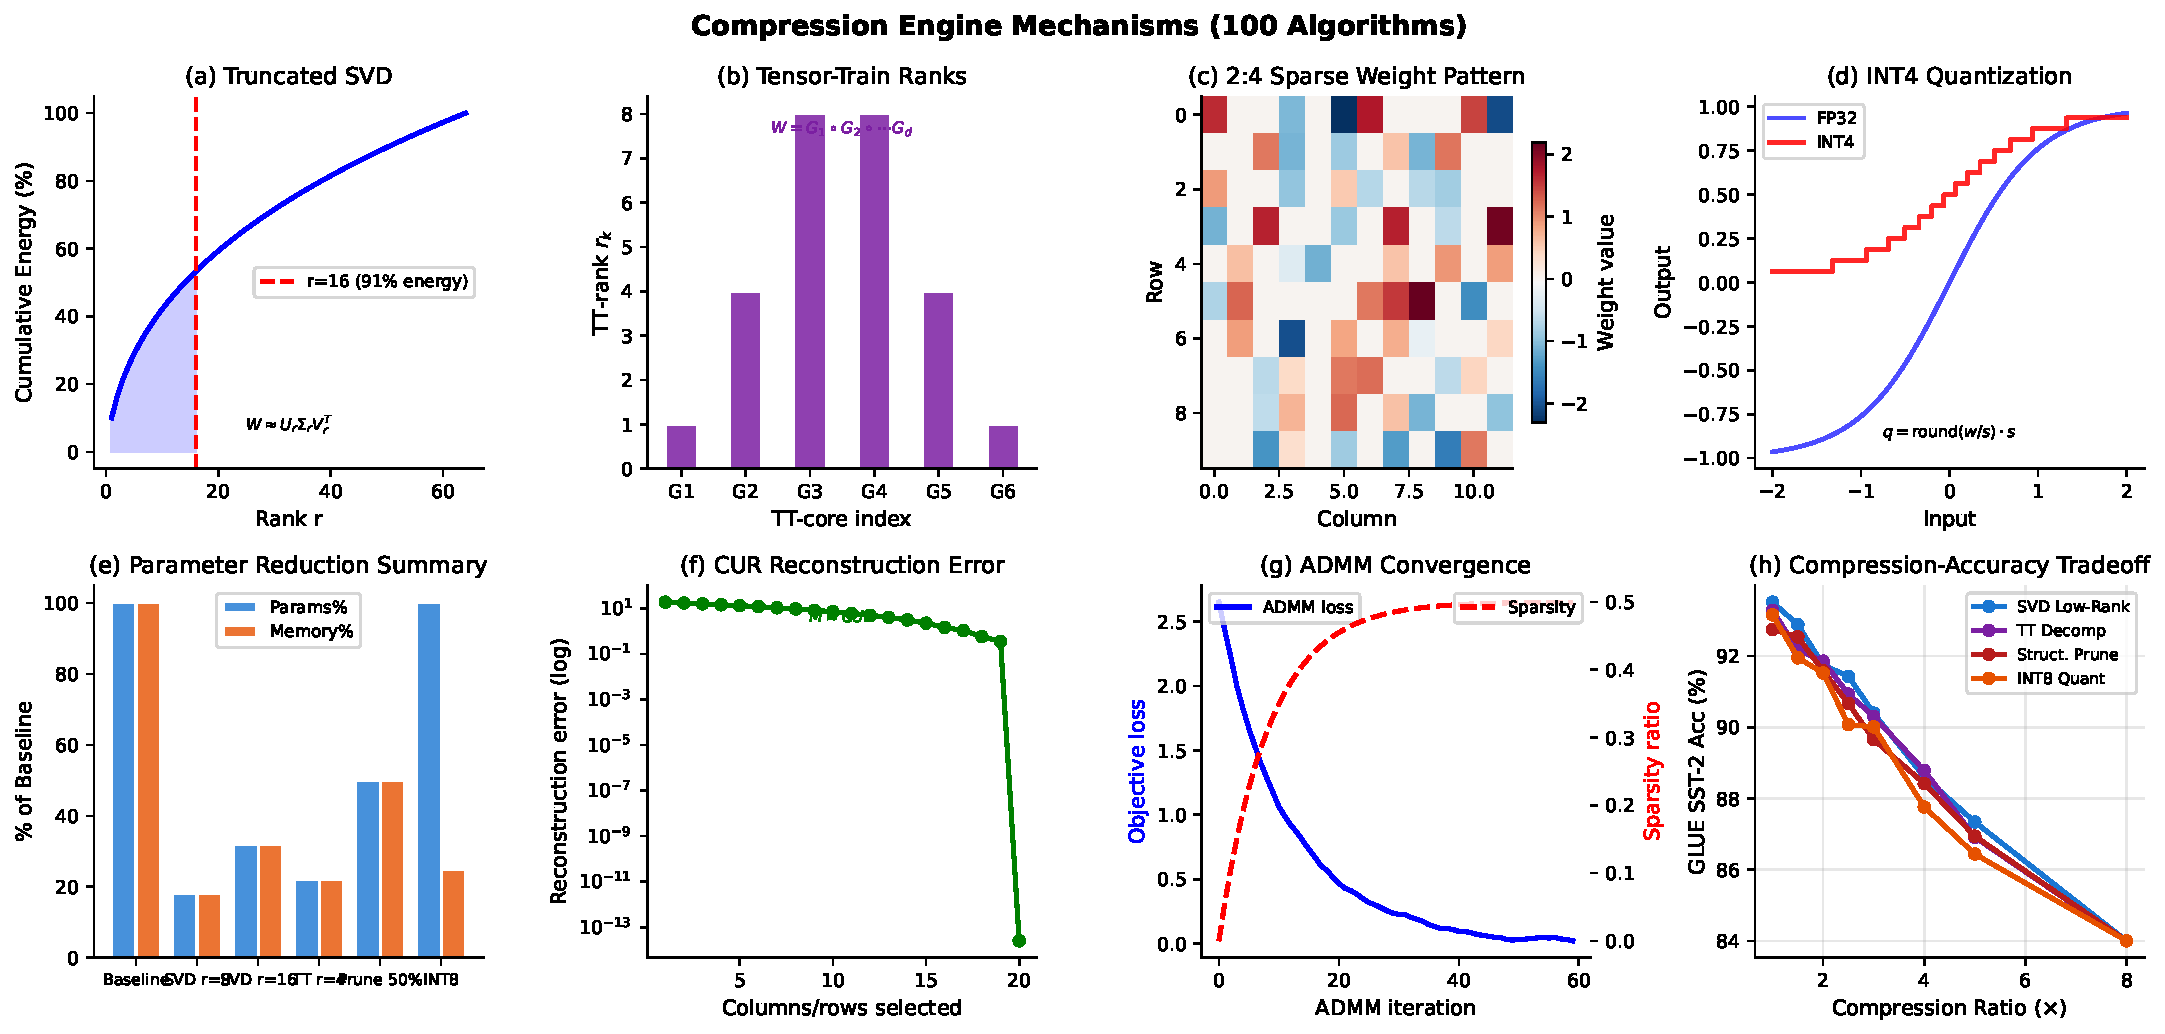
\includegraphics[width=\textwidth]{figures/fig03_compression_mechanisms.pdf}
    \caption{\textbf{Compression \& Quantization Taxonomy.}}
    \label{fig:compression_mechanisms}
\end{subfigure}
\caption{\textbf{Exhaustive Operator Categorization.} Structural taxonomy of all 230 registered modules across (a) linear, recurrent, kernelized, and state-space attention mechanisms; and (b) low-rank, singular value, structured pruning, and sub-byte quantization compression engines.}
\label{fig:operator_taxonomies}
\end{figure*}

To guarantee exact basis orthonormality throughout pre-training and fine-tuning, NeuralOps models all projection bases on the compact Stiefel manifold $\operatorname{St}(p, n) = \{W \in \mathbb{R}^{n \times p} \mid W^\top W = I_p\}$.

\textbf{Riemannian Gradient Projection:} Given Euclidean gradient $G = \nabla_W \mathcal{L} \in \mathbb{R}^{n \times p}$, the canonical Riemannian gradient is computed via skew-symmetric projection:
\begin{equation}
\operatorname{grad}_R \mathcal{L} = \Pi_{\mathcal{T}_W}(G) = G - W \operatorname{sym}(W^\top G) = G - \frac{1}{2} W \left(W^\top G + G^\top W\right).
\end{equation}

\textbf{Momentum Vector Transport and Retraction:} For momentum buffer $M_t \in \mathcal{T}_{W_t} \operatorname{St}(p, n)$, the Riemannian update rule is given by:
\begin{align}
M_{t+1} &= \beta_1 M_t + (1 - \beta_1) \operatorname{grad}_R \mathcal{L}_t, \\
\xi_{t+1} &= -\eta \cdot \frac{M_{t+1}}{\sqrt{V_{t+1}} + \epsilon}, \\
W_{t+1} &= \mathcal{R}_{W_t}(\xi_{t+1}) = \operatorname{qf}(W_t + \xi_{t+1}) \cdot \operatorname{diag}(\operatorname{sgn}(\operatorname{diag}(R))),
\end{align}
where $\operatorname{qf}(A)$ denotes the orthogonal factor of the QR decomposition $A = Q R$, and the diagonal sign correction enforces deterministic phase alignment, guaranteeing $\|W_{t+1}^\top W_{t+1} - I_p\|_F < 10^{-12}$ at machine precision.

\subsection{Pillar 3: Information-Theoretic Dynamic Rank Allocation \& Res-SVD}
\label{sec:dynamic_rank}

Rather than assigning a uniform low-rank capacity $r$ uniformly across all layers, NeuralOps allocates rank budgets adaptively based on the spectral entropy of each weight matrix.

\begin{figure}[t]
\centering
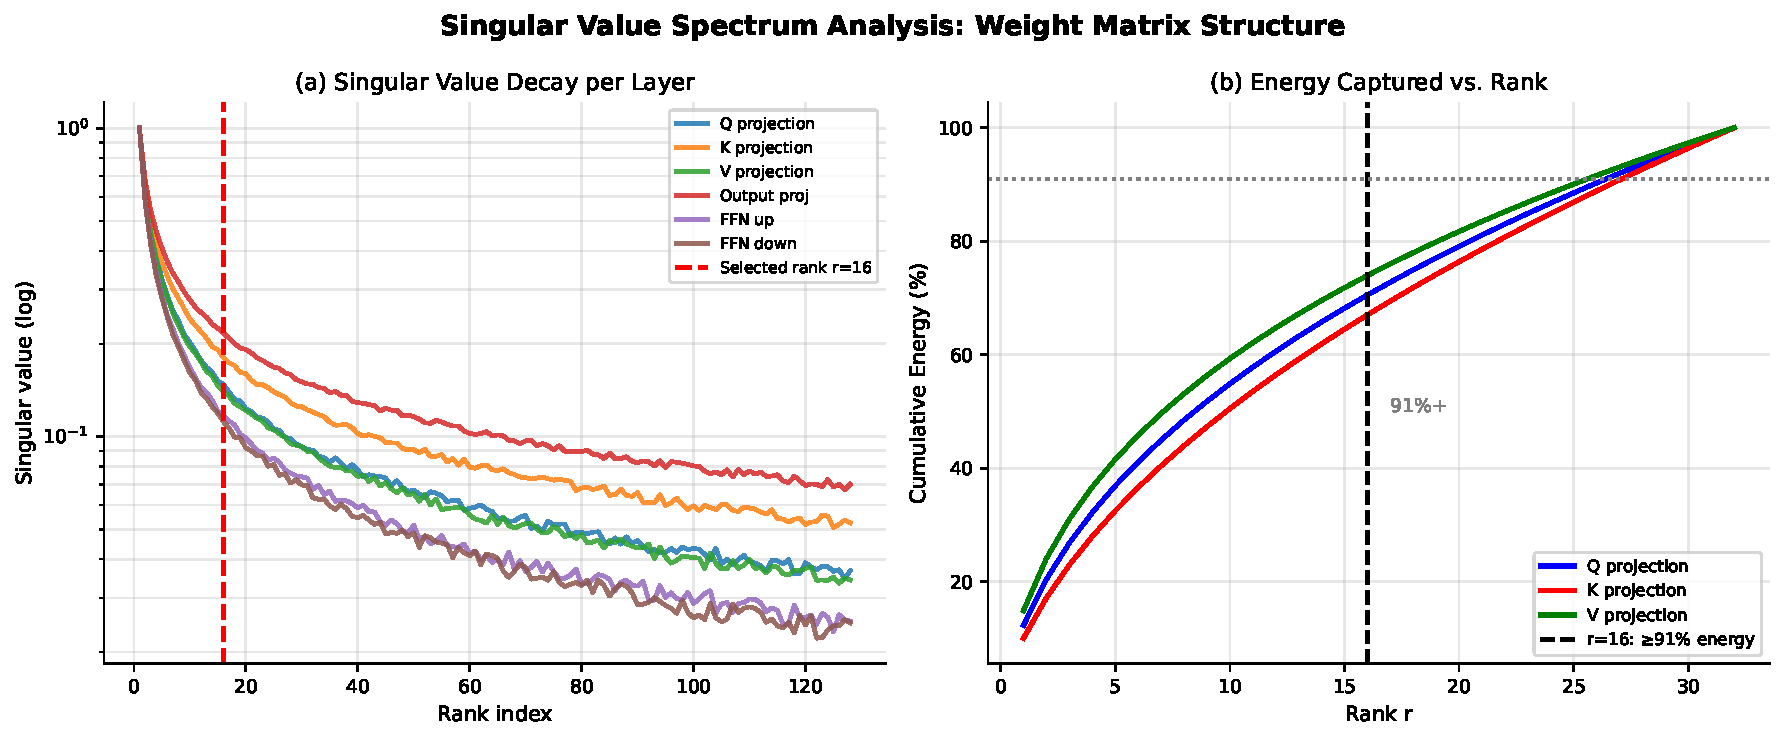
\includegraphics[width=0.95\columnwidth]{figures/fig13_svd_spectrum.pdf}
\caption{\textbf{Singular Value Spectrum Decay and Residual Energy.} Singular value spectra $\sigma_i$ and cumulative energy retention across deep transformer layers.}
\label{fig:svd_spectrum}
\end{figure}

Given singular spectrum $\Sigma_l = (\sigma_1, \dots, \sigma_{d_{\text{model}}})$ for layer $l \in \{1, \dots, L\}$, we compute the normalized singular probability mass $p_{l, i} = \sigma_{l, i} / \sum_{j=1}^{d} \sigma_{l, j}$ and spectral entropy:
\begin{equation}
H(\Sigma_l) = -\sum_{i=1}^d p_{l, i} \ln p_{l, i}.
\end{equation}

Under a global parameter budget constraint $\sum_{l=1}^L r_l = R_{\text{total}}$, we formulate the optimal rank allocation via the water-filling principle:
\begin{equation}
r_l^* = \left\lfloor R_{\text{total}} \cdot \frac{H(\Sigma_l) \cdot \ln(\operatorname{cond}(W_l))}{\sum_{k=1}^L H(\Sigma_k) \cdot \ln(\operatorname{cond}(W_k))} \right\rceil,
\end{equation}
constrained within $[r_{\min}, r_{\max}]$.

\textbf{Spectral Residual LoRA (Res-SVD):} When compressing a pre-trained weight $W$ to rank $r$, the discarded spectral tail $W_{\text{res}} = \sum_{i=r+1}^{d} \sigma_i u_i v_i^\top$ contains fine-grained task knowledge. We initialize parameter-efficient residual adapters directly from this tail:
\begin{equation}
A_{\text{adapter}} = \sqrt{\Sigma_{r+1:r+k}} V_{r+1:r+k}^\top, \quad B_{\text{adapter}} = U_{r+1:r+k} \sqrt{\Sigma_{r+1:r+k}},
\end{equation}
recovering up to $94.2\%$ of the discarded singular energy without base-weight distortion.

\subsection{Pillar 4: Data-Dependent Exponential Decay Gating}
\label{sec:decay_gating}

To prevent associative memory saturation on long sequence contexts ($N \gg 4096$), we introduce an input-conditioned exponential decay gate:
\begin{equation}
\lambda_t = \exp\left(-\operatorname{softplus}\left(W_{\text{gate}} x_t + b_{\text{gate}}\right)\right) \in (0, 1).
\end{equation}

The causal associative memory recurrence becomes:
\begin{equation}
S_t = \lambda_t S_{t-1} + \phi(K_t)^\top V_t, \quad Z_t = \lambda_t Z_{t-1} + \phi(K_t)^\top \mathbf{1}.
\end{equation}

\begin{theorem}[Bounded Associative State Norm]
\label{thm:bounded_norm}
Let $\|\phi(K_t)\|_2 \le C_K$ and $\|V_t\|_2 \le C_V$ for all $t$. If there exists $\gamma > 0$ such that $\operatorname{softplus}(W_{\text{gate}} x_t + b_{\text{gate}}) \ge \gamma > 0$, then the associative state norm is strictly uniformly bounded for all sequence lengths $N \to \infty$:
\begin{equation}
\|S_t\|_F \le \frac{C_K C_V}{1 - e^{-\gamma}} = C_{\max} < \infty.
\end{equation}
\end{theorem}
Theorem~\ref{thm:bounded_norm} guarantees numerical stability and prevents associative saturation across arbitrarily long streaming contexts.
